\documentclass[12pt]{report}

%% Useful packages
\usepackage[a4paper,top=3cm,bottom=3cm,left=3.7cm,right=2.5cm,marginparwidth=1.75cm,headheight=22pt]{geometry}
\usepackage[hidelinks]{hyperref} %you can remove for red bounding box around links
\usepackage{amsmath}
\usepackage{cite}
\usepackage{courier}
\usepackage{minted} % For highlighted source code
\usepackage[titletoc]{appendix}
\usepackage[export]{adjustbox}
\usepackage[nottoc,notlot,notlof]{tocbibind}
\usepackage[labelfont=bf, textfont=bf]{caption}
\usepackage{graphicx}
\usepackage{booktabs}
\usepackage[bottom]{footmisc}
\usepackage{hyperref}
\usepackage{float}
\usepackage{setspace}
\usepackage{subfigure}
\usepackage{setspace}
\usepackage{lipsum}
\usepackage{fancyhdr} % Fancy header
\usepackage{url}
\usepackage{tabularx}
\usepackage[utf8]{inputenc}
\usepackage{mathptmx} %Times Font
\usepackage{csquotes}

%==== Header and Footer configure ====
% Define the plain pagestyle used by most chapters
\fancypagestyle{plain}{
\fancyhf{} % Clear header footer
\fancyhead[R]{\bf \small \textsl{\nouppercase{\leftmark}} \vspace{0.1in}}
\fancyfoot[R]{\thepage}
% Set the right side of the footer to be the page number
\renewcommand{\headrulewidth}{2pt}
}

%==== Overall Config ====
\setlength{\parindent}{0in} % Set paragraph indent as 0
% \setlength{\fboxsep}{-0.3in}%
\setlength{\fboxrule}{0.5pt} % Set the bounding box around the image as 0.5pt
\pagestyle{plain}
% \renewcommand{\chaptermark}[1]{\markboth{#1}{}}% Comment this line to use header "Chapter 1. Literature View"; otherwise header is "Literature View"



\begin{document}
\fontdimen2\font=0.5em% inter word space
%==== FRONT PART====
\begin{titlepage}

\begin{figure}[h!]
\centering

\includegraphics[width=0.5\textwidth, right]{Title/logo.png}
\caption*{}
\label{fig:entropy} 
\end{figure}

\vspace{0.5in}

\centering
\Huge{\textbf{Your Title of the Dissertation\\Also Second Line}}\\[2.0in]

\large{\textit{\textbf{John Doe}}} \\[0.2in]
\large{\textit{\textbf{Supervisor: John Doe}}} \\[0.8in]

\vspace{1.5in}

\normalsize{\textbf{June - 2022}}\\[0.2in]

\normalsize{\textbf{A dissertation submitted to the Institute of Information and Communication Technology in partial fulfilment of
the requirements for the degree of BSc (Hons) Multimedia in Software Development}}\\[0.2in]


\end{titlepage}
\newpage % Coverpage

%\begingroup
%\let\cleardoublepage\clearpage
\pagenumbering{roman}

%=== Authorship Statement ===
\newpage

\chapter*{\centering Authorship Statement}
\markboth{Authorship Statement}{}
% \vspace{-0.3in}

\begin{spacing}{1.5}
\setlength{\parskip}{0.3in}

\addcontentsline{toc}{chapter}{Authorship Statement}

This dissertation is based on the results of research carried out by myself, is my
own composition, and has not been previously presented for any other certified
or uncertified qualification.

The research was carried out under the supervision of (name of dissertation tutor
–Title, Name and surname)

\vspace{2.5cm}

\begin{center}
	\makebox[4cm]{\dotfill}  \hfill \makebox[4cm]{\dotfill}\\
	\makebox[4cm]{Date}      \hfill \makebox[4cm]{Signature}
\end{center}
\end{spacing}
\newpage
%=== END OF ABSTRACT ===

%=== Copyright Statement ===
\newpage

\chapter*{\centering Copyright Statement}
\markboth{Copyright Statement}{}
% \vspace{-0.3in}

\begin{spacing}{1.5}
\setlength{\parskip}{0.3in}

\addcontentsline{toc}{chapter}{Copyright Statement}

In submitting this dissertation to the MCAST Institute of Information and Com-
munication Technology, I understand that I am giving permission for it to be
made available for use in accordance with the regulations of MCAST and the
Library and Learning Resource Centre. I accept that my dissertation may be
made publicly available at MCAST’s discretion.

\vspace{2.5cm}

\begin{center}
	\makebox[4cm]{\dotfill}  \hfill \makebox[4cm]{\dotfill}\\
	\makebox[4cm]{Date}      \hfill \makebox[4cm]{Signature}
\end{center}
\end{spacing}
\newpage
%=== END OF ABSTRACT ===

%=== FRONT PART ===
%=== ABSTRCT ===
\newpage

\chapter*{\centering Abstract}
\markboth{Abstract}{}
% \vspace{-0.3in}

\begin{spacing}{1.5}
\setlength{\parskip}{0.3in}

\addcontentsline{toc}{chapter}{Abstract}

This section should clearly state what the study is about, summarizing how it was carried out and what the results were. References are not to be included in the abstract. It should present only the essentials of the work in general. 400-500 words.

\par
\textbf{Keywords:} Dissertation, keywords.
\end{spacing}
\newpage
%=== END OF ABSTRACT ===

%=== FRONT PART ===
%=== ACKNOWLEDGEMENT ===

%\begin{center}
\chapter*{\centering Acknowledgements}
\markboth{Acknowledgements}{}
\begin{spacing}{1.5}
\setlength{\parskip}{0.3in}
%\end{center}
\addcontentsline{toc}{chapter}{Acknowledgements}

The list of people that the Student would like to thank on the completion of the dissertation. For example ‘Mr Name Surname, who supported me during my dissertation work as my tutor’.

\end{spacing}
\newpage
%=== END OF ACKNOWLEDGEMENT  ===


\renewcommand*\contentsname{\centering Table of Contents}
\tableofcontents
\newpage



%=== FRONT PART ===
%=== ACRONYMS ===
%\begin{center}
\chapter*{\centering Acronyms}
\markboth{Acronyms}{}
\begin{spacing}{1.5}
\setlength{\parskip}{0.3in}
%\end{center}
\addcontentsline{toc}{chapter}{Acronyms}

\begin{table}[ht]
\centering
% \resizebox{0.8\textwidth}{!}{% Uncomment to set fixed width
\begin{tabular}{ll}
\textbf{NN} & Neural Network \\
\textbf{ML} & Machine Learning \\
\textbf{DL} & Deep Learning \\
\textbf{FCN} & Fully Convolutional Network \\
\textbf{CNN} & Convolutional Neural Network \\
\textbf{RCNN} & Region Based Convolutional Neural Network \\
\textbf{DCNN} & Deep Convolutional Neural Network
\end{tabular}%
% }
\end{table}

\end{spacing}
\newpage
%=== END OF ACRONYMS ===

%=== FRONT PART ===
%=== SYMBOLS ===
%\begin{center}
\chapter*{\centering Symbols}
\markboth{Symbols}{}
\begin{spacing}{1.5}
\setlength{\parskip}{0.3in}
%\end{center}
\addcontentsline{toc}{chapter}{Symbols}

\begin{table}[ht]
\centering
% \resizebox{0.8\textwidth}{!}{% Uncomment to set fixed width
\begin{tabular}{ll}
\textbf{$\Pi$} & An Pi Symbol\\
\textbf{$\beta$} & An Beta Symbol\\
\textbf{$\sigma$} & An Sigma Symbol\\
\textbf{$\alpha$} & Another Alpha Symbol\\
\end{tabular}%
% }
\end{table}

\end{spacing}
\newpage
%=== END OF ACKNOWLEDGEMENT  ===



\renewcommand{\listfigurename}{\centering List of Figures}
\listoffigures
\addcontentsline{toc}{chapter}{Lists of Figures}
\newpage

\renewcommand{\listtablename}{\centering List of Tables}
\listoftables 
\addcontentsline{toc}{chapter}{Lists of Tables}
\newpage

%\endgroup

%==== MAIN PART ====

\pagenumbering{arabic}
%=== CHAPTER ONE (1) ===
%=== INTRODUCTION ===

\chapter{Introduction}
\begin{spacing}{1.5}
\setlength{\parskip}{0.3in}

In this section, the Student is expected to state clearly:
a) the ‘problem’ or ‘question’ being researched;
b) why this topic was chosen;
c) what motivated the Student to choose this topic;
d) why did the Student investigate it the way they did;
e) what problem did the Student wish to explore;
f) what is the context for the research?
(500-1000 words)

\section{Sub-chapter One}


Background goes here. Also you can put in some references~\cite{ronneberger2015unet}.

Another example of citations \cite{latex2e,ronneberger2015unet}.

Here is a sample of table in \autoref{tabelsample}

\begin{table}[ht]
\centering
\caption{A table without vertical lines.}
\label{tabelsample}
\begin{tabular}[t]{lcc}
\toprule
&Treatment A&Treatment B\\
\midrule
John Smith&1&2\\
Jane Doe&--&3\\
Mary Johnson&4&5\\
\bottomrule
\end{tabular}
\end{table}%

Use  \texttt{$\backslash$newpage} to force start a new page.

\newpage
Use  \texttt{$\backslash$enquote} for double-quotes. \enquote{This is a sample quote.}

Also can try to refer to this image in \autoref{fig:boundingboxexample}. Notice that the \texttt{.eps} and \texttt{.pdf} format vector graphs are favoured, because:

\begin{enumerate}
    \item they can be zoomed-in to check the detail.
    \item text in such formats are search-able.
\end{enumerate}


\begin{figure}[ht]
\centering
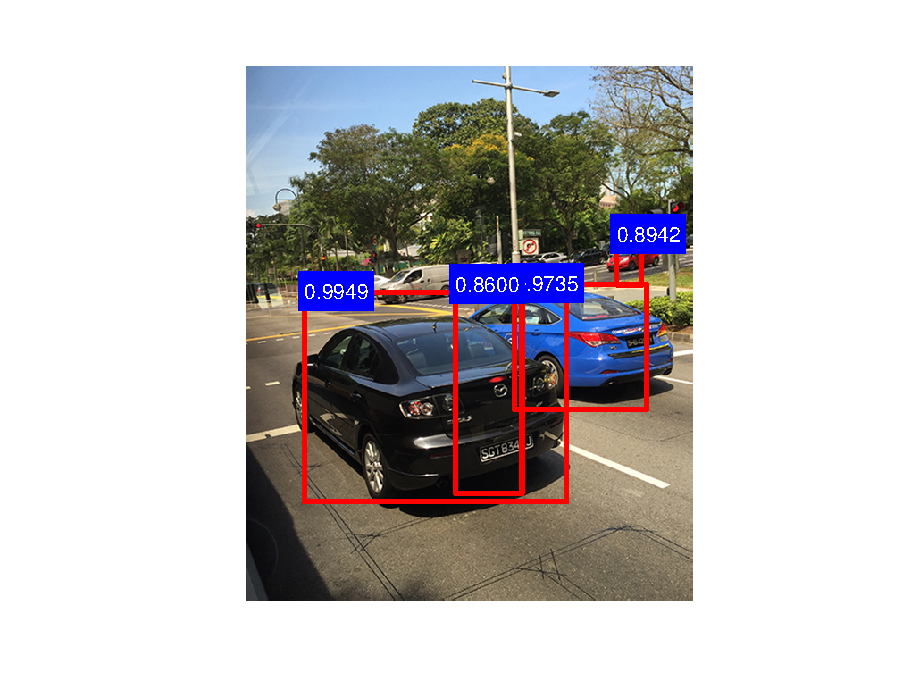
\includegraphics[width=4in, fbox]{Chapter1/boundingbox.eps}
\caption{Bounding-box example of cars.}
\label{fig:boundingboxexample} 
\end{figure}

Try to insert a math equation as in \autoref{eq:euler}. If you wanna try the in-line mathematical, here is a sample $\alpha = \pi \cdot \frac{1}{\Theta}$.

\begin{equation}
\label{eq:euler}
    e^{ix}= \cos{x} + i \sin{x}
\end{equation}

Also here is a sample for footnote and hyperlink url\footnote{\url{https://github.com/doem97}}. 

When mention some file formats can use \texttt{music.mp3}, \texttt{latex.pdf}, etc.




\section{Sub-chapter Two}

Contrary to popular belief, Lorem Ipsum is not simply random text. It has roots in a piece of classical Latin literature from 45 BC, making it over 2000 years old. Richard McClintock, a Latin professor at Hampden-Sydney College in Virginia, looked up one of the more obscure Latin words, consectetur, from a Lorem Ipsum passage, and going through the cites of the word in classical literature, discovered the undoubtable source. Lorem Ipsum comes from sections 1.10.32 and 1.10.33 of de Finibus Bonorum et Malorum (The Extremes of Good and Evil) by Cicero, written in 45 BC. This book is a treatise on the theory of ethics, very popular during the Renaissance. The first line of Lorem Ipsum, \enquote{Lorem ipsum dolor sit amet}.., comes from a line in section 1.10.32.

It is a long established fact that a reader will be distracted by the readable content of a page when looking at its layout. The point of using Lorem Ipsum is that it has a more-or-less normal distribution of letters, as opposed to using 'Content here, content here', making it look like readable English. Many desktop publishing packages and web page editors now use Lorem Ipsum as their default model text, and a search for 'lorem ipsum' will uncover many web sites still in their infancy. Various versions have evolved over the years, sometimes by accident, sometimes on purpose (injected humour and the like).

\section{Sub-chapter Three}

Vivamus eget odio tellus. Nam libero augue, eleifend molestie est eu, tempus vehicula magna. Sed dignissim imperdiet urna, non viverra risus blandit in. In lacinia aliquet leo, ut interdum ipsum ornare sed. Praesent ac fringilla justo. Vivamus pharetra non ipsum eget semper. In hac habitasse platea dictumst. Donec neque lectus, ultricies id massa posuere, sodales interdum ante. Sed et nunc vitae urna ornare porttitor nec vitae urna. Curabitur sit amet luctus urna. Nulla porta malesuada rutrum. Pellentesque vitae velit sed odio tincidunt iaculis. Nulla facilisi.

\section{Sub-chapter Four}

Phasellus elit nulla, dapibus id aliquam vitae, eleifend id diam. Aenean a porta arcu. Sed eget sem sed odio maximus lobortis. Aliquam id lobortis felis, non molestie nisi. Curabitur accumsan efficitur suscipit. Nulla facilisi. Pellentesque lorem odio, congue at metus sit amet, vehicula hendrerit turpis. Phasellus lectus ipsum, imperdiet a augue in, tempus finibus ante.

Aenean ornare augue quis urna mollis, vel suscipit leo efficitur. Nunc tellus massa, lobortis et dui id, semper dignissim quam. Duis mollis auctor dui ac lacinia. Praesent quis molestie erat, nec bibendum tellus. Quisque consequat pretium turpis gravida semper. Donec ac velit tempor, viverra tellus quis, hendrerit augue. Praesent posuere ullamcorper dui, eu finibus nisi gravida non. Vivamus hendrerit neque at dolor fringilla, id pretium turpis pulvinar. Nunc et leo volutpat, commodo magna non, pretium sapien. Proin dignissim, nibh at tincidunt rutrum, ante tellus interdum arcu, eget ultricies urna odio sit amet mauris. Integer pulvinar leo congue diam imperdiet vestibulum.

\newpage
\section{Sub-chapter Five}
In euismod mauris tortor, non sodales tortor consectetur dapibus. Aenean dignissim ultricies lacus id malesuada. Cras laoreet luctus ligula, id dictum purus ultrices faucibus. Orci varius natoque penatibus et magnis dis parturient montes, nascetur ridiculus mus. Nulla at ante sed ex venenatis pretium in ut lorem. Cras condimentum pretium dignissim. Maecenas ac tempor ipsum, eu blandit enim. Mauris pharetra, justo in iaculis tincidunt, neque nisl eleifend tortor, in volutpat libero erat vitae lorem. Suspendisse dignissim quis eros eget varius. In porttitor augue vel ligula varius, a tincidunt eros gravida. Etiam eget porta ipsum.

Ut venenatis lectus at nisi consectetur volutpat. Vivamus vehicula a odio ac scelerisque. Fusce tincidunt diam eu orci pellentesque, eu vehicula felis posuere. Mauris tempus dignissim leo, vitae eleifend justo ultrices eget. Fusce volutpat suscipit urna. Curabitur ultrices nibh dolor, quis ultricies risus condimentum quis. Nulla non nulla quis odio laoreet pulvinar non eu turpis. Interdum et malesuada fames ac ante ipsum primis in faucibus. Morbi odio nisi, hendrerit id laoreet nec, fringilla quis neque. Quisque non nisl vitae leo vulputate fringilla. Sed blandit lectus dui, vestibulum tempor elit laoreet vel. Nullam at magna ut elit dapibus gravida vitae eu dolor. Aliquam ut odio ullamcorper, venenatis elit eget, feugiat arcu. Nunc nibh lacus, dapibus condimentum neque vitae, tempus eleifend ex. Integer sit amet volutpat orci, quis tristique augue. Nam sit amet dolor dignissim, luctus justo sit amet, luctus velit.

\end{spacing}
%=== END OF CHAPTER ONE ===
\newpage



%=== CHAPTER TWO (2) ===
%=== Literature Review ===

\chapter{Literature Review}
\begin{spacing}{1.5}
\setlength{\parskip}{0.3in}

\section{Overview}

The main purpose of a literature review is to show the reader that the Student studied and analyzed viewpoints of other researchers on the problem under consideration. A literature review is not just a summary of the books read but rather a thorough analysis of other viewpoints on the problem being analysed. (2,000 – 4,000 words)


\section{One}
In euismod mauris tortor, non sodales tortor consectetur dapibus. Aenean dignissim ultricies lacus id malesuada. Cras laoreet luctus ligula, id dictum purus ultrices faucibus. Orci varius natoque penatibus et magnis dis parturient montes, nascetur ridiculus mus. Nulla at ante sed ex venenatis pretium in ut lorem. Cras condimentum pretium dignissim. Maecenas ac tempor ipsum, eu blandit enim. Mauris pharetra, justo in iaculis tincidunt, neque nisl eleifend tortor, in volutpat libero erat vitae lorem. Suspendisse dignissim quis eros eget varius. In porttitor augue vel ligula varius, a tincidunt eros gravida. Etiam eget porta ipsum.

Ut venenatis lectus at nisi consectetur volutpat. Vivamus vehicula a odio ac scelerisque. Fusce tincidunt diam eu orci pellentesque, eu vehicula felis posuere. Mauris tempus dignissim leo, vitae eleifend justo ultrices eget. Fusce volutpat suscipit urna. Curabitur ultrices nibh dolor, quis ultricies risus condimentum quis. Nulla non nulla quis odio laoreet pulvinar non eu turpis. Interdum et malesuada fames ac ante ipsum primis in faucibus. Morbi odio nisi, hendrerit id laoreet nec, fringilla quis neque. Quisque non nisl vitae leo vulputate fringilla. Sed blandit lectus dui, vestibulum tempor elit laoreet vel. Nullam at magna ut elit dapibus gravida vitae eu dolor. Aliquam ut odio ullamcorper, venenatis elit eget, feugiat arcu. Nunc nibh lacus, dapibus condimentum neque vitae, tempus eleifend ex. Integer sit amet volutpat orci, quis tristique augue. Nam sit amet dolor dignissim, luctus justo sit amet, luctus velit.

\begin{figure}[ht]
\centering
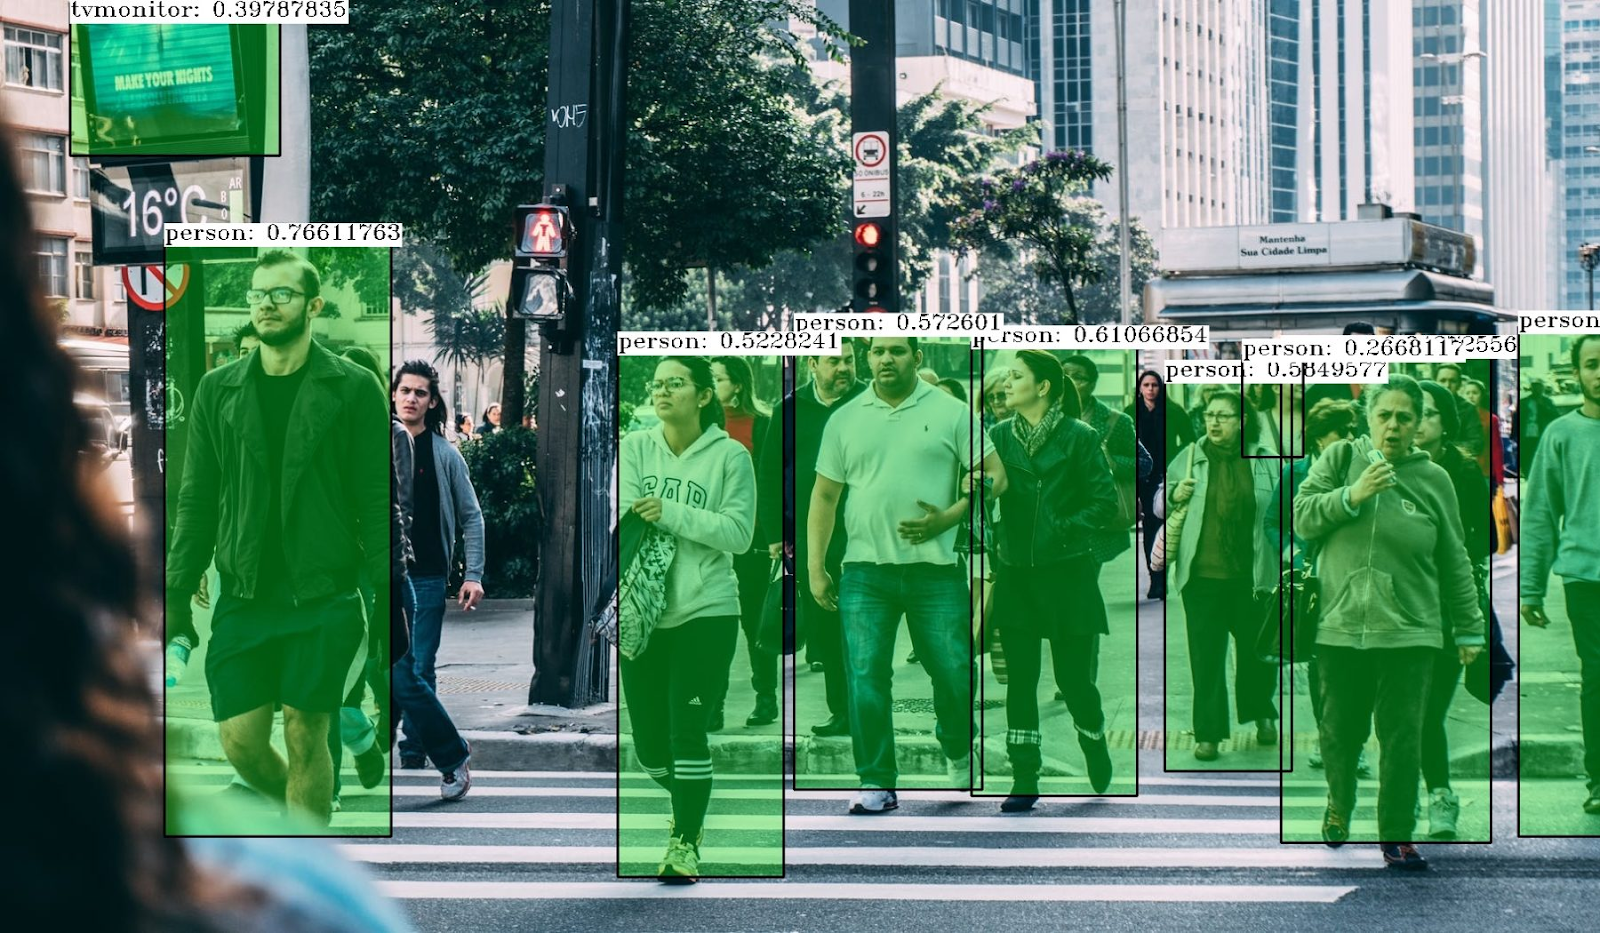
\includegraphics[width=5in, fbox]{Chapter1/opencv.png}
\caption{Machine Learning.}
\label{fig:opencvexample} 
\end{figure}

\section{Two}
In euismod mauris tortor, non sodales tortor consectetur dapibus. Aenean dignissim ultricies lacus id malesuada. Cras laoreet luctus ligula, id dictum purus ultrices faucibus. Orci varius natoque penatibus et magnis dis parturient montes, nascetur ridiculus mus. Nulla at ante sed ex venenatis pretium in ut lorem. Cras condimentum pretium dignissim. Maecenas ac tempor ipsum, eu blandit enim. Mauris pharetra, justo in iaculis tincidunt, neque nisl eleifend tortor, in volutpat libero erat vitae lorem. Suspendisse dignissim quis eros eget varius. In porttitor augue vel ligula varius, a tincidunt eros gravida. Etiam eget porta ipsum.

Ut venenatis lectus at nisi consectetur volutpat. Vivamus vehicula a odio ac scelerisque. Fusce tincidunt diam eu orci pellentesque, eu vehicula felis posuere. Mauris tempus dignissim leo, vitae eleifend justo ultrices eget. Fusce volutpat suscipit urna. Curabitur ultrices nibh dolor, quis ultricies risus condimentum quis. Nulla non nulla quis odio laoreet pulvinar non eu turpis. Interdum et malesuada fames ac ante ipsum primis in faucibus. Morbi odio nisi, hendrerit id laoreet nec, fringilla quis neque. Quisque non nisl vitae leo vulputate fringilla. Sed blandit lectus dui, vestibulum tempor elit laoreet vel. Nullam at magna ut elit dapibus gravida vitae eu dolor. Aliquam ut odio ullamcorper, venenatis elit eget, feugiat arcu. Nunc nibh lacus, dapibus condimentum neque vitae, tempus eleifend ex. Integer sit amet volutpat orci, quis tristique augue. Nam sit amet dolor dignissim, luctus justo sit amet, luctus velit.

\section{Three}
In euismod mauris tortor, non sodales tortor consectetur dapibus. Aenean dignissim ultricies lacus id malesuada. Cras laoreet luctus ligula, id dictum purus ultrices faucibus. Orci varius natoque penatibus et magnis dis parturient montes, nascetur ridiculus mus. Nulla at ante sed ex venenatis pretium in ut lorem. Cras condimentum pretium dignissim. Maecenas ac tempor ipsum, eu blandit enim. Mauris pharetra, justo in iaculis tincidunt, neque nisl eleifend tortor, in volutpat libero erat vitae lorem. Suspendisse dignissim quis eros eget varius. In porttitor augue vel ligula varius, a tincidunt eros gravida. Etiam eget porta ipsum.


\subsection{Four}
Ut venenatis lectus at nisi consectetur volutpat. Vivamus vehicula a odio ac scelerisque. Fusce tincidunt diam eu orci pellentesque, eu vehicula felis posuere. Mauris tempus dignissim leo, vitae eleifend justo ultrices eget. Fusce volutpat suscipit urna. Curabitur ultrices nibh dolor, quis ultricies risus condimentum quis. Nulla non nulla quis odio laoreet pulvinar non eu turpis. Interdum et malesuada fames ac ante ipsum primis in faucibus. Morbi odio nisi, hendrerit id laoreet nec, fringilla quis neque. Quisque non nisl vitae leo vulputate fringilla. Sed blandit lectus dui, vestibulum tempor elit laoreet vel. Nullam at magna ut elit dapibus gravida vitae eu dolor. Aliquam ut odio ullamcorper, venenatis elit eget, feugiat arcu. Nunc nibh lacus, dapibus condimentum neque vitae, tempus eleifend ex. Integer sit amet volutpat orci, quis tristique augue. Nam sit amet dolor dignissim, luctus justo sit amet, luctus velit.

%=== END OF CHAPTER TWO ===
\end{spacing}
\newpage

%=== CHAPTER THREE (3) ===
%=== (Actual work done and contribution, including literature survey) ===

\chapter{Research Methodology}
\begin{spacing}{1.5}
\setlength{\parskip}{0.3in}
%  (Actual work done and contribution, including literature survey)


\section{One}

It presents the chosen research methods and explains why these methods are effective. (1,500 – 3,000 words)

\section{Two}


\section{Three}


%=== END OF CHAPTER THREE ===
\end{spacing}
\newpage

%=== CHAPTER FOUR (4) ===
%=== Test and Experiments ===

\chapter{Analysis of Results and Discussion}
\begin{spacing}{1.5}
\setlength{\parskip}{0.3in}

\section{One}
This section includes critical discussion about the Student’s findings and shows how these findings support the original objectives laid out for the dissertation, which may be partially or
fully achieved, or even exceeded. The Student may also include new areas of an investigation prompted by developments in the research dissertation. Above all, it is required to present strong arguments which show how findings may offer a valid contribution to the development of the subject of the selected research area or issues related to it. (3,000 – 4,000 words)

\section{Two}

\section{Three}


%=== END OF CHAPTER FOUR ===
\end{spacing}
\newpage

%=== CHAPTER FIVE (5) ===
%=== Discussion ===

\chapter{Conclusions and Recommendations}
\begin{spacing}{1.5}
\setlength{\parskip}{0.3in}

\section{One}

In this chapter, the Student has to evaluate the significance of the work done and give recommendations for any further investigations. (1,000 – 3,000 words)

\section{Two}

\section{Three}


%=== END OF CHAPTER FIVE ===
\end{spacing}
\newpage


%==== ENDING PART ===

\renewcommand\bibname{References}
\bibliographystyle{unsrt}
\begin{spacing}{1.5}
\bibliography{Ref/References}
\end{spacing}
\newpage

%=== APPENDIX ===

\begin{appendices}
\label{cha:appendices}

\chapter{Introduction of Appendix}
\markboth{Appendix A}{} % For appendix first (affects header)
\begin{spacing}{1.5}

Interview summaries, sample questionnaires, and references should be placed in this section.For easier referencing, figures, tables, graphs, photos, diagrams, etc., should be inserted within
the main text such as the literature review, the experimental process or procedure, the results and discussion chapters. Appendices are usually used to present further details about the results. Appendices may be a compulsory part of a dissertation, but they are not treated as part of the dissertation for purposes
of assessing the dissertation. So any material which is significant to judging the quality of the dissertation or of the project as a whole should be in the main body of the dissertation (main text), and not in appendices.

\end{spacing}

\chapter{Sample Code}
\markboth{Appendix B}{} % For appendix second, etc.. 

You can share your GitHub link. Below shows how to insert highlighted source code from the source file.

\inputminted[
tabsize=4, % change this to set the spacing of tab
breaklines, % automatically wrap the code
fontsize=\scriptsize % Can be \footnotesize, \small, \normalsize etc
]{python}{Appendix/sample.py}

\end{appendices}
%==== END OF ALL ===
\end{document}
